\documentclass{beamer}
\usepackage{lmodern}% http://ctan.org/pkg/lm
\usepackage{amsmath}
\usepackage{color}
\usepackage{graphics}
\usepackage{tikz}
\usetikzlibrary{%
  fit,
  arrows,%
  shapes.misc,% wg. rounded rectangle
  shapes.arrows,%
  chains,%
  matrix,%
  positioning,% wg. " of "
  scopes,%
  decorations.pathmorphing,% /pgf/decoration/random steps | erste Graphik
  shadows,
  automata
}
\setbeamercolor{bgcolor}{fg=black,bg=white}

\begin{document}
\title{A Contribution to Rating and Recommendation Systems: Concepts, Development and Evaluation}   
\author{Oliver Diestel} 
\date{\today} 

\frame{\titlepage} 

%\frame{\frametitle{Inhaltsverzeichnis}\tableofcontents} 

\section{The Problem} 
\frame{\frametitle{The Problem}
  The problem: Recommending user generated content.\\
  %Challenges: Recommending items that the user is interested in\\
  %creating implicit recommendations for this task\\
  %match user generated content with the content of the website that the recommendation displays.\\
  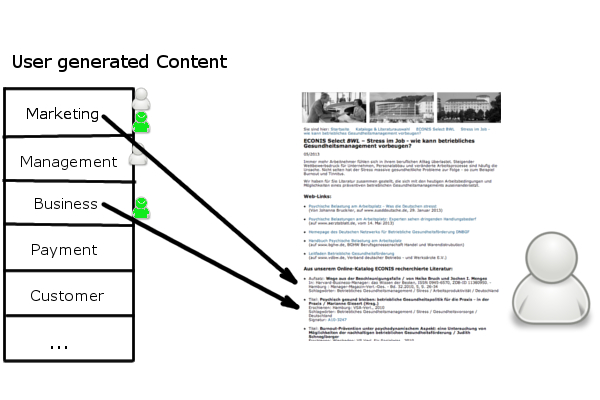
\includegraphics[width=300px]{usercontent.jpg} \\
}

\frame{\frametitle{Challenges} 
\vspace{0.2cm}

\includegraphics[width=300px]{question.png} \\

% The items that are recommended in this thesis are questions and answers\\
% The content is user generated therefore no information about the quality of the content.\\
% No information about the subject of the content.

%My part is to bring user relevant information that fits the current subject onto a website.
}
% \frame{\frametitle{Beginning}
% Getting to know the content.\\
% First step.\\
% Generate user ratings for the content.\\
% => Opens the possibility of collaborative filtering the content and thus finding the good content for recommendations.


% %After every new concept answer the question what do we have now
% }

\section{Rating}
\frame{\frametitle{Rating}
%explain the research, the best are user spends and user scrolls with about 70% correlation with the explicit ratings
Based on the work of Claypool et al 2001\\
\begin{itemize}
\item The time a user spends on a website 
\item The time the cursor is in motion 
\item The number of mouse clicks
\item The time a user scrolls
\end{itemize}
}
\frame{\frametitle{Rating}
Claypool et al 2001\\
    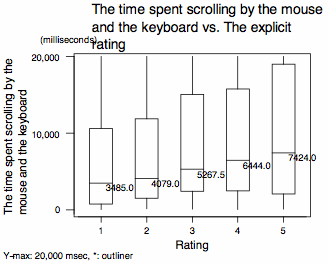
\includegraphics[width=280px]{image/scroll} 

%explain the images describe the idea of generating a implicit rating scale out of these findings
}
\frame{\frametitle{Rating}
Claypool et al 2001\\
   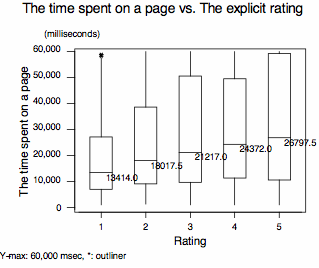
\includegraphics[width=280px]{image/time} 

%explain the images describe the idea of generating a implicit rating scale out of these findings
}

% \frame{\frametitle{Rating}
% \begin{definition}[Truncated Mean]
%   Let $n \in \mathbb{N}$, V be a set of sorted numbers and p be a percentage with $0 \leq p < 0.5$.
%   Let $k = np$ be the trimmed value, $r = n - 2k$ be the remaining values, $v_j \in V$ and $j \in \mathbb{N}$.
%   Then the following formula represents the truncated mean.
%   \begin{displaymath}
%     Truncated Mean = \sum_{j=k+1}^{n-k}{v_j} \cdot \frac{1}{r}
%   \end{displaymath}
% \end{definition}

% }

\frame{\frametitle{Rating}
\begin{displaymath}
  p = \frac{Time Spend}{Truncated Mean Of Time Spend}
\end{displaymath}

\scriptsize
  \begin{center}
    \begin{tabular}{| l | l | l | l | l |}
      \hline
      \multicolumn{5}{|c|}{Rating for Time a user spends} \\ 
      \hline \hline
      1 & 2 & 3 & 4 & 5 \\ \hline
      $0\% \leq p < 76\%$ & $76\% \leq p < 95\%$ & $95\% \leq p < 110\%$ & $110\% \leq p < 125\%$& -\\ \hline
    \end{tabular} 
  \end{center}
  \normalsize

}

\frame{\frametitle{Rating}
\begin{displaymath}
  p = \frac{Time Scrolled}{Truncated Mean Of Time Scrolled}
\end{displaymath}

\tiny
  \begin{center}
    \begin{tabular}{| l | l | l | l | l |}
      \hline
      \multicolumn{5}{|c|}{Rating for Time a user scrolls} \\ 
      \hline \hline
      1 & 2 & 3 & 4 & 5 \\ \hline
      $0\% \leq p < 69\%$ & $69\% \leq p < 86\%$ & $86\% \leq p < 108\%$ & $108\% \leq p < 129\%$& $129\% \leq p$\\ \hline
    \end{tabular} 
  \end{center}
  \normalsize

}



\section{Tagging}
\frame{\frametitle{Tagging}
Find the keywords that describe the question.
\pause
\begin{itemize}
\item STW Thesaurus for Economics %, tripple store
  \pause
\item Computing Levenshtein distance: Calculate the distance between two words.\\
  Example:\\
  Libraries, Librar\textcolor{red}{y}\\
  Distance: 3
\end{itemize}
}

\frame{\frametitle{Levenshtein Automata}
  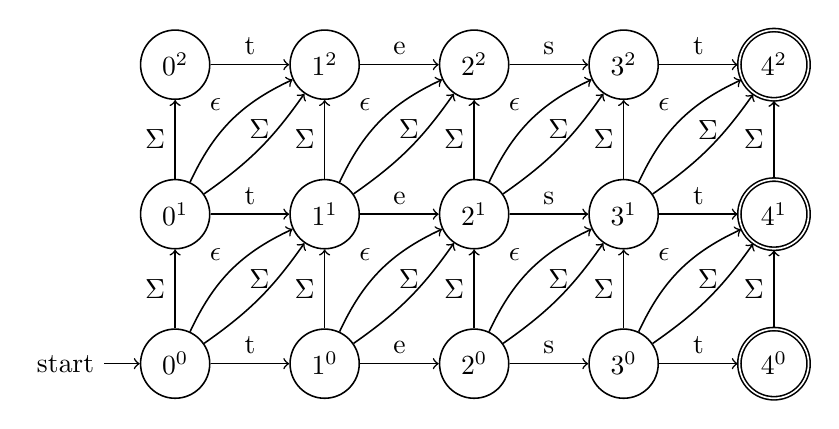
\begin{tikzpicture}[->,auto,line width=0.2mm] 
    %0,0 row
    \node[state] (q_2) {$0^2$}; 
    \node[state] (q_1) [below =of q_2] {$0^1$}; 
    \node[state,initial] (q_0) [below =of q_1] {$0^0$}; 

    %1,0 row t
    \node[state] (q_5) [right =of q_2] {$1^2$}; 
    \node[state] (q_4) [right =of q_1] {$1^1$}; 
    \node[state] (q_3) [right =of q_0] {$1^0$}; 

    %2,0 row e
    \node[state] (q_8) [right =of q_5] {$2^2$}; 
    \node[state] (q_7) [right =of q_4] {$2^1$}; 
    \node[state] (q_6) [right =of q_3] {$2^0$};

    %3,0 row s
    \node[state] (q_11) [right =of q_8] {$3^2$}; 
    \node[state] (q_10) [right =of q_7] {$3^1$}; 
    \node[state] (q_9) [right =of q_6] {$3^0$};

    %4,0 row t
    \node[state, accepting] (q_14) [right =of q_11] {$4^2$}; 
    \node[state, accepting] (q_13) [right =of q_10] {$4^1$}; 
    \node[state, accepting] (q_12) [right =of q_9] {$4^0$};

    %path deletion 0,0
    \path[->] 
    (q_0) edge node {$\Sigma$} (q_1)
    (q_1) edge node {$\Sigma$} (q_2);
    %path 0,0 -> 1,0
    \path[->] 
    %correct path
    (q_0) edge  node {t} (q_3)
    (q_1) edge  node  {t} (q_4)
    (q_2) edge  node  {t} (q_5)

    %insertion substitution
    (q_0) edge[bend right=10]  node[above,midway] {$\Sigma$} (q_4)
    (q_0) edge[bend left=20]  node  {$\epsilon$} (q_4)


    (q_1) edge[bend right=10]  node[above,midway] {$\Sigma$} (q_5)
    (q_1) edge[bend left=20]  node  {$\epsilon$} (q_5);

    %path deletion 1,0
    \path[->] 
    (q_3) edge node {$\Sigma$} (q_4)
    (q_4) edge node {$\Sigma$} (q_5);

    %path 1,0 -> 2,0
    \path[->] 
    %correct path
    (q_3) edge  node {e} (q_6)
    (q_4) edge  node  {e} (q_7)
    (q_5) edge  node  {e} (q_8)

    %insertion substitution
    (q_3) edge[bend right=10]  node[above,midway] {$\Sigma$} (q_7)
    (q_3) edge[bend left=20]  node  {$\epsilon$} (q_7)


    (q_4) edge[bend right=10]  node[above,midway] {$\Sigma$} (q_8)
    (q_4) edge[bend left=20]  node  {$\epsilon$} (q_8);


    %path deletion 2,0
    \path[->] 
    (q_6) edge node {$\Sigma$} (q_7)
    (q_7) edge node {$\Sigma$} (q_8);

    %path 1,0 -> 2,0
    \path[->] 
    %correct path
    (q_6) edge  node {s} (q_9)
    (q_7) edge  node  {s} (q_10)
    (q_8) edge  node  {s} (q_11)

    %insertion substitution
    (q_6) edge[bend right=10]  node[above,midway] {$\Sigma$} (q_10)
    (q_6) edge[bend left=20]  node  {$\epsilon$} (q_10)


    (q_7) edge[bend right=10]  node[above,midway] {$\Sigma$} (q_11)
    (q_7) edge[bend left=20]  node  {$\epsilon$} (q_11);

    %path deletion 3,0
    \path[->] 
    (q_9) edge node {$\Sigma$} (q_10)
    (q_10) edge node {$\Sigma$} (q_11);

    %path 3,0 -> 4,0
    \path[->] 
    %correct path
    (q_9) edge  node {t} (q_12)
    (q_10) edge  node  {t} (q_13)
    (q_11) edge  node  {t} (q_14)

    %insertion substitution
    (q_9) edge[bend right=10]  node[above,midway] {$\Sigma$} (q_13)
    (q_9) edge[bend left=20]  node  {$\epsilon$} (q_13)


    (q_10) edge[bend right=10]  node[above,midway] {$\Sigma$} (q_14)
    (q_10) edge[bend left=20]  node  {$\epsilon$} (q_14);

    %path deletion 3,0
    \path[->] 
    (q_12) edge node {$\Sigma$} (q_13)
    (q_13) edge node {$\Sigma$} (q_14);


  \end{tikzpicture}

}

\frame{\frametitle{Levenshtein Automata}
  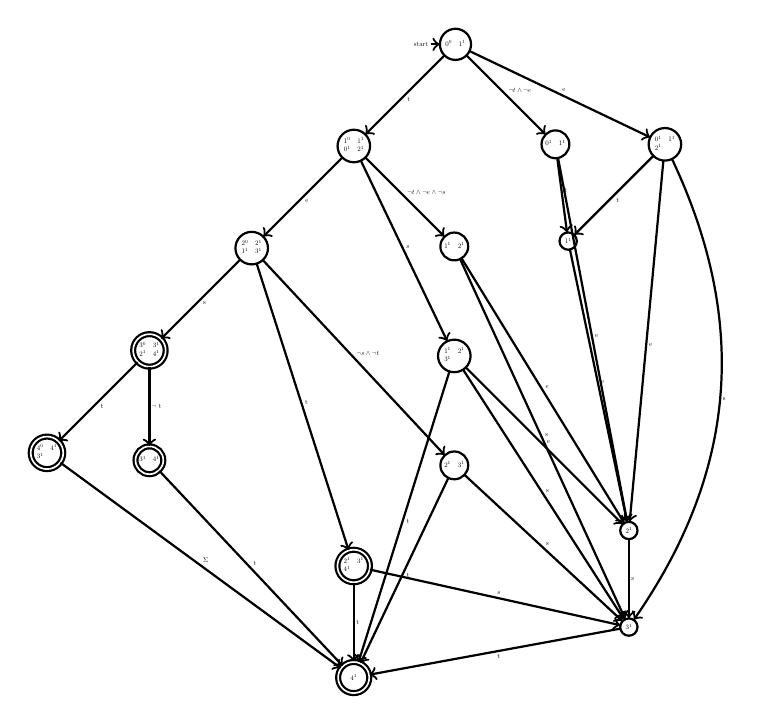
\begin{tikzpicture}[->,auto,line width=0.2mm, thick,scale=0.25, every node/.style={scale=0.25}]
    \node[state,initial, minimum size=4.5em] (0_0-1_1) {$\begin{matrix} 0^0 & 1^1 \end{matrix}$}; 
    %correct path
     \node[state] (1_0-1_1-0_1-2_1) [below left=of 0_0-1_1] {$\begin{matrix} 1^0 & 1^1\\ 0^1 & 2^1 \end{matrix}$}; 
     \node[state] (2_0-2_1-1_1-3_1) [below left=of 1_0-1_1-0_1-2_1] {$\begin{matrix} 2^0 & 2^1\\ 1^1 & 3^1 \end{matrix}$}; 
     \node[state, accepting] (3_0-3_1-2_1-4_1) [below left=of 2_0-2_1-1_1-3_1] {$\begin{matrix} 3^0 & 3^1\\ 2^1 & 4^1 \end{matrix}$}; 

     \node[state, accepting] (4_0-4_1-3_1) [below left=of 3_0-3_1-2_1-4_1] {$\begin{matrix} 4^0 & 4^1\\ 3^1 \end{matrix}$}; 

     %first not t,e
     \node[state] (0_1-1_1) [below right=of 0_0-1_1] {$\begin{matrix} 0^1 & 1^1\end{matrix}$}; 

     %first e
     \node[state] (0_1-1_1-2_1) [right=of 0_1-1_1] {$\begin{matrix} 0^1 & 1^1\\ 2^1 \end{matrix}$}; 

      %q1 edges
     \node[state] (1_1-2_1) [below right=of 1_0-1_1-0_1-2_1] {$\begin{matrix} 1^1 & 2^1 \end{matrix}$}; 
     \node[state] (1_1-2_1-3_1) [below =of 1_1-2_1] {$\begin{matrix} 1^1 & 2^1 \\ 3^1 \end{matrix}$}; 

     %elementar
     \node[state] (1_1) [below left=of 0_1-1_1-2_1] {$1^1$}; 
     \node[state] (2_1) [below right=8em of 1_1-2_1-3_1] {$2^1$}; 
     \node[state] (3_1) [below =of 2_1] {$3^1$}; 



     \node[state, accepting] (3_1-4_1) [below =of 3_0-3_1-2_1-4_1] {$\begin{matrix} 3^1 & 4^1 \end{matrix}$}; 

     \node[state] (2_1-3_1) [below =of 1_1-2_1-3_1] {$\begin{matrix} 2^1 & 3^1 \end{matrix}$}; 
     \node[state, accepting] (2_1-3_1-4_1) [below left=of 2_1-3_1] {$\begin{matrix} 2^1 & 3^1\\ 4^1 \end{matrix}$}; 
     \node[state, accepting, minimum size=4.5em] (4_1) [below =of 2_1-3_1-4_1] {$4^1$}; 
     \path[->]
     (0_0-1_1) edge node {$\neg t \wedge \neg e$} (0_1-1_1)
     (2_0-2_1-1_1-3_1) edge node {$\neg s \land \neg t$} (2_1-3_1)
     (2_0-2_1-1_1-3_1) edge node {t} (2_1-3_1-4_1)
     (0_0-1_1) edge node {e} (0_1-1_1-2_1)
     (1_0-1_1-0_1-2_1) edge node {$\neg t \wedge \neg e \wedge \neg s$} (1_1-2_1)
     (1_0-1_1-0_1-2_1) edge node {s} (1_1-2_1-3_1)
     (0_1-1_1) edge  node {t} (1_1)
     (0_1-1_1) edge  node {e} (2_1)
     (1_1) edge  node {e} (2_1)
     (2_1) edge  node {s} (3_1)
     (3_1) edge  node {t} (4_1)
     (1_1-2_1) edge  node {e} (2_1)
     (1_1-2_1) edge  node {s} (3_1)
     (3_0-3_1-2_1-4_1) edge node {$\neg$ t} (3_1-4_1)
     (3_1-4_1) edge node {t} (4_1)
     (0_0-1_1) edge  node {t} (1_0-1_1-0_1-2_1)
     (1_0-1_1-0_1-2_1) edge  node  {e} (2_0-2_1-1_1-3_1)
     (2_0-2_1-1_1-3_1) edge  node  {s} (3_0-3_1-2_1-4_1)
     (3_0-3_1-2_1-4_1) edge  node  {t} (4_0-4_1-3_1)
     (2_1-3_1-4_1) edge  node {t} (4_1)
     (2_1-3_1-4_1) edge  node {s} (3_1)
     (2_1-3_1) edge  node {s} (3_1)
     (2_1-3_1) edge  node {t} (4_1)
     (0_1-1_1-2_1) edge  node {t} (1_1)
     (0_1-1_1-2_1) edge  node {e} (2_1)
     (0_1-1_1-2_1) edge[bend left=30]  node {s} (3_1)
     (1_1-2_1-3_1) edge  node {e} (2_1)
     (1_1-2_1-3_1) edge  node {s} (3_1)
     (1_1-2_1-3_1) edge  node {t} (4_1)
     (4_0-4_1-3_1) edge  node  {$\Sigma$} (4_1);


  \end{tikzpicture}
  %each word from stw is read into each automata
  %if word is in final state use word as tag
  %the levenshtein automata is not knew however the use case is

}
\frame{\frametitle{Levenshtein Automata}
  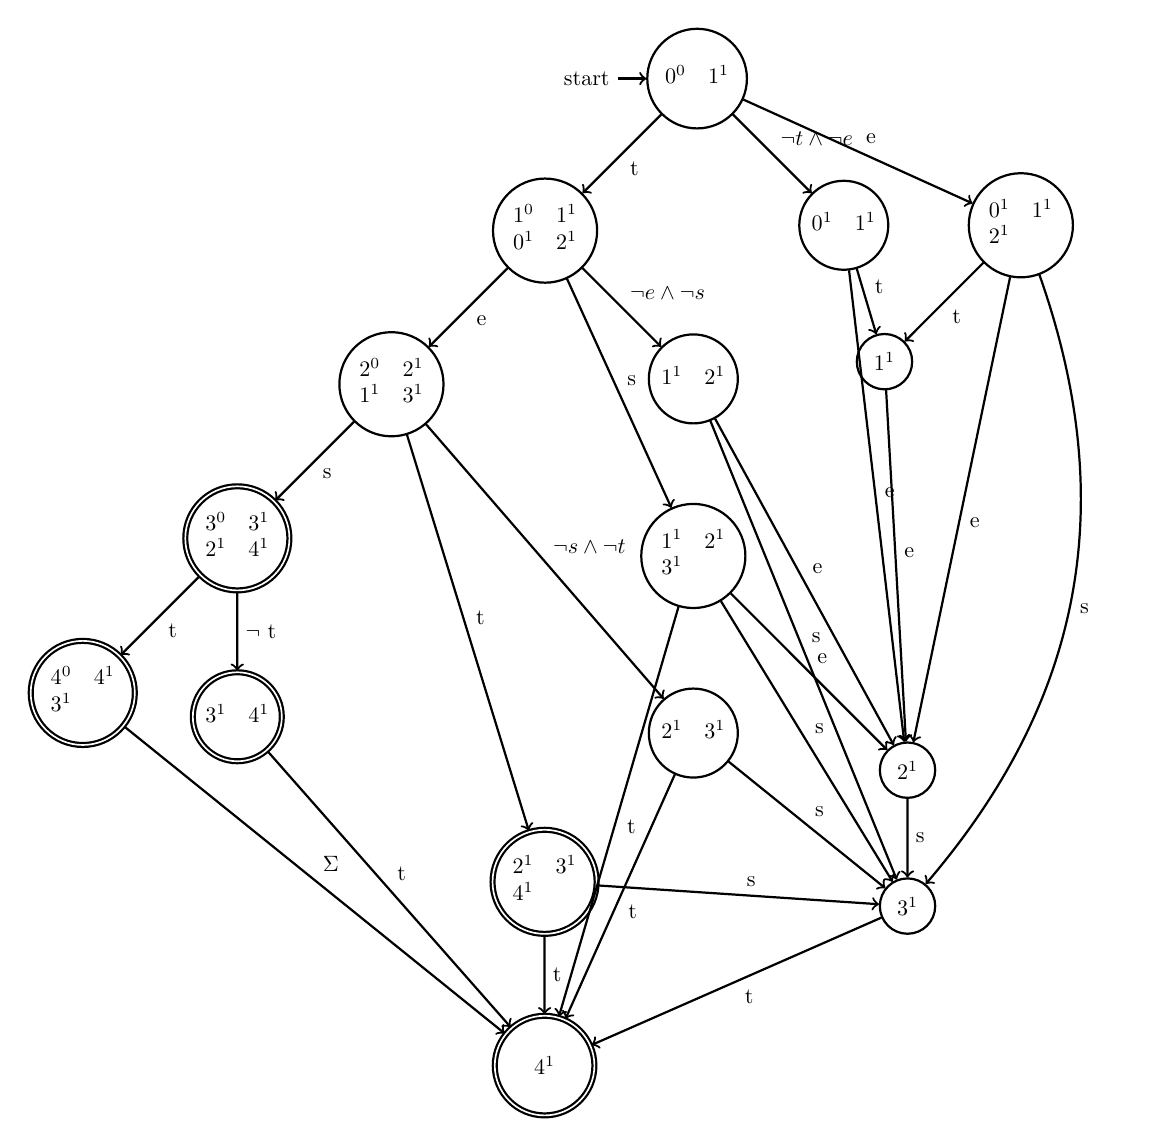
\begin{tikzpicture}[->,auto,line width=0.2mm, thick,scale=0.8, every node/.style={scale=0.8}]
    \node[state,initial, minimum size=4.5em] (0_0-1_1) {$\begin{matrix} 0^0 & 1^1 \end{matrix}$}; 
    %correct path
     \node[state] (1_0-1_1-0_1-2_1) [below left=of 0_0-1_1] {$\begin{matrix} 1^0 & 1^1\\ 0^1 & 2^1 \end{matrix}$}; 
     \node[state] (2_0-2_1-1_1-3_1) [below left=of 1_0-1_1-0_1-2_1] {$\begin{matrix} 2^0 & 2^1\\ 1^1 & 3^1 \end{matrix}$}; 
     \node[state, accepting] (3_0-3_1-2_1-4_1) [below left=of 2_0-2_1-1_1-3_1] {$\begin{matrix} 3^0 & 3^1\\ 2^1 & 4^1 \end{matrix}$}; 

     \node[state, accepting] (4_0-4_1-3_1) [below left=of 3_0-3_1-2_1-4_1] {$\begin{matrix} 4^0 & 4^1\\ 3^1 \end{matrix}$}; 

     %first not t,e
     \node[state] (0_1-1_1) [below right=of 0_0-1_1] {$\begin{matrix} 0^1 & 1^1\end{matrix}$}; 

     %first e
     \node[state] (0_1-1_1-2_1) [right=of 0_1-1_1] {$\begin{matrix} 0^1 & 1^1\\ 2^1 \end{matrix}$}; 

      %q1 edges
     \node[state] (1_1-2_1) [below right=of 1_0-1_1-0_1-2_1] {$\begin{matrix} 1^1 & 2^1 \end{matrix}$}; 
     \node[state] (1_1-2_1-3_1) [below =of 1_1-2_1] {$\begin{matrix} 1^1 & 2^1 \\ 3^1 \end{matrix}$}; 

     %elementar
     \node[state] (1_1) [below left=of 0_1-1_1-2_1] {$1^1$}; 
     \node[state] (2_1) [below right=8em of 1_1-2_1-3_1] {$2^1$}; 
     \node[state] (3_1) [below =of 2_1] {$3^1$}; 



     \node[state, accepting] (3_1-4_1) [below =of 3_0-3_1-2_1-4_1] {$\begin{matrix} 3^1 & 4^1 \end{matrix}$}; 

     \node[state] (2_1-3_1) [below =of 1_1-2_1-3_1] {$\begin{matrix} 2^1 & 3^1 \end{matrix}$}; 
     \node[state, accepting] (2_1-3_1-4_1) [below left=of 2_1-3_1] {$\begin{matrix} 2^1 & 3^1\\ 4^1 \end{matrix}$}; 
     \node[state, accepting, minimum size=4.5em] (4_1) [below =of 2_1-3_1-4_1] {$4^1$}; 
     \path[->]
     (0_0-1_1) edge node {$\neg t \wedge \neg e$} (0_1-1_1)
     (2_0-2_1-1_1-3_1) edge node {$\neg s \land \neg t$} (2_1-3_1)
     (2_0-2_1-1_1-3_1) edge node {t} (2_1-3_1-4_1)
     (0_0-1_1) edge node {e} (0_1-1_1-2_1)
     (1_0-1_1-0_1-2_1) edge node {$\neg e \wedge \neg s$} (1_1-2_1)
     (1_0-1_1-0_1-2_1) edge node {s} (1_1-2_1-3_1)
     (0_1-1_1) edge  node {t} (1_1)
     (0_1-1_1) edge  node {e} (2_1)
     (1_1) edge  node {e} (2_1)
     (2_1) edge  node {s} (3_1)
     (3_1) edge  node {t} (4_1)
     (1_1-2_1) edge  node {e} (2_1)
     (1_1-2_1) edge  node {s} (3_1)
     (3_0-3_1-2_1-4_1) edge node {$\neg$ t} (3_1-4_1)
     (3_1-4_1) edge node {t} (4_1)
     (0_0-1_1) edge  node {t} (1_0-1_1-0_1-2_1)
     (1_0-1_1-0_1-2_1) edge  node  {e} (2_0-2_1-1_1-3_1)
     (2_0-2_1-1_1-3_1) edge  node  {s} (3_0-3_1-2_1-4_1)
     (3_0-3_1-2_1-4_1) edge  node  {t} (4_0-4_1-3_1)
     (2_1-3_1-4_1) edge  node {t} (4_1)
     (2_1-3_1-4_1) edge  node {s} (3_1)
     (2_1-3_1) edge  node {s} (3_1)
     (2_1-3_1) edge  node {t} (4_1)
     (0_1-1_1-2_1) edge  node {t} (1_1)
     (0_1-1_1-2_1) edge  node {e} (2_1)
     (0_1-1_1-2_1) edge[bend left=30]  node {s} (3_1)
     (1_1-2_1-3_1) edge  node {e} (2_1)
     (1_1-2_1-3_1) edge  node {s} (3_1)
     (1_1-2_1-3_1) edge  node {t} (4_1)
     (4_0-4_1-3_1) edge  node  {$\Sigma$} (4_1);


  \end{tikzpicture}
  %each word from stw is read into each automata
  %if word is in final state use word as tag
  %the levenshtein automata is not knew however the use case is

}

\frame{\frametitle{Maximum Distance for Words}

   \begin{center}
    \begin{tabular}{| l | l | l | l | }
      \hline
      Length & $\leq$ 3 & $\leq$ 5 &  6 $\leq$\\ \hline
      Distance & 0 & 1 & 3 \\ \hline
    \end{tabular} 
  \end{center}
  \pause
  Problem Feminina with \emph{e-plural: Hand H\"ande} \\
  \pause
  \emph{Maskulina und Neutra mit er-Plural 3 \"anderungen Wurm W\"urmer Substantive mit er plural Fass F\"asser} \\

 Based on \emph{Die Pluralbildung im Deutschen: Eine Untersuchung an Hand der Optimalit\"atstheorie: "German Noun Plural reconsidered" von Dieter Wunderlich}
}

\frame{\frametitle{Tagging Evaluation}
% \begin{center}
%   \begin{tabular}{| l | l | l | l | l | }
%     \hline
%     \multicolumn{5}{|c|}{Rating Algorithm Evaluation} \\ 
%     \hline \hline
%     Scroll Time & Scroll Rating & Time Spend & Time Rating & Total Rating \\ \hline
%     3.559 & 1 & 14.012 & 1 & 1 \\ \hline
%     3.249 & 1 & 21.603 & 3 & 2 \\ \hline
%     3.355 & 1 & 25.497 & 4 & 3 \\ \hline
%     5.077 & 3 & 13.414 & 1 & 2 \\ \hline
%     5.342 & 3 & 21.217 & 3 & 3 \\ \hline
%     5.287 & 3 & 26.797 & 4 & 4 \\ \hline
%     7.374 & 5 & 12.113 & 1 & 3 \\ \hline
%     7.504 & 5 & 20.917 & 3 & 4 \\ \hline
%     7.431 & 5 & 24.797 & 4 & 5 \\ \hline
%   \end{tabular} 
% \end{center}

  \begin{center}
    \resizebox{\columnwidth}{!}{%
    
    \begin{tabular}{| l | l | l | l | l | l |}
      \hline
      \multicolumn{6}{|c|}{Tagging Algorithm Evaluation} \\ 
      \hline \hline
      Words & STW & Non Matching & Matched Words & Levenshtein Time & Total Time \\ \hline
      1 & 1 & 0 & 2 & 0.099 & 14.481 \\ \hline
      10 & 3 & 7 & 3 & 0.2843 & 20.348 \\ \hline
      100 & 30 & 70 & 54 & 0.4751 & 79.9616\\ \hline
      1000 & 300 & 700 & 470 & 2.5606 & 777.4643\\ \hline
    \end{tabular} 
  }
  \end{center}


}




\section{Recommendation}


\frame{\frametitle{Item-Based Algorithm}
%To find similar users we need as much user/item ratings as possible so we would like to guess as much ratings as possible.
  \begin{tabular}{c c c c c c}
   &Item1 & Item2 & Item3 & Item4 & Item5 \\ 
  User1 & 5 & 3 & 4 & 4 & ?\\  
  User2 & ? & 1 & ? & 3 & 3\\ 
  User3 & 4 & ? & 4 & 3 & 5\\ 
  User4 & 3 & 3 & ? & 5 & 4\\ 
  User5 & 1 & 5 & 5 & 2 & 1\\ 
  \end{tabular}

\pause
\begin{block}{Cosinus Similarity} %change to adjusted cosine similarity
\begin{math}
  a = [a_1, a_2, \dots, a_n], b = [b_1, b_2, \dots, b_n] \\
  sim(\overrightarrow{a}, \overrightarrow{b}) = {\overrightarrow{a} \cdot \overrightarrow{b} \over ||\overrightarrow{a}||\cdot||\overrightarrow{b}||} = \frac{\sum_{i = 1}^{n}\overrightarrow{a_i}\overrightarrow{b_i}}{\sqrt{\sum_{i = 1}^n \overrightarrow{a_i}^2} \sqrt{\sum_{i = 1}^n\overrightarrow{b_i}^2 }}

\end{math}
\end{block}

  Take the differences of the average rating behaviour of the user into account.

  \begin{block}{Adjusted Cosinus Similarity}
  \begin{math}
    sim(a, b) = {\sum_{u \in U}(r_{u, a} - \overline{r_u})(r_{u,b} - \overline{r_u}) \over \sqrt{\sum_{u \in U}(r_{u,a} - \overline{r_u})^2} \sqrt{\sum_{u \in U}(r_{u,b} - \overline{r_u})^2 }}
  \end{math}
  \end{block}
}
\frame{\frametitle{Predictions}
%Calculate predictions for similar items.\\
  \begin{block}{Prediction}
    User u, Item p, Rating r_{u, p}\\
    \begin{math}
      pred(u, p) = {\sum_{i \in ratedItems(u)} sim(i, p) \cdot r_{u, i} \over \sum_{i \in ratedItems(u)} sim(i, p)}
    \end{math}
  \end{block}
  %well known concept the new idea is to use these predictions to fill the rating matrix

%Fill recommendation vector of each user with similar item ratings 
}

\frame{\frametitle{Singular Value Decomposition}

  %Now we would like to find similar users with our matrix
  \begin{center}
    ~
    \begin{beamercolorbox}[rounded=true, center, shadow=false,wd=6cm]{bgcolor}
      \begin{math}
        M = \begin{pmatrix} m_{11} & m_{12} & m_{13} \\ m_{21} & m_{22} & m_{23} \\ m_{31} & m_{32} & m_{33}\end{pmatrix}
      \end{math}
    \end{beamercolorbox}
    ~
  \end{center}

  Create a SVD with the matrix 
  \begin{math}
    M = U \cdot \Sigma \cdot V^t
  \end{math}
   %explanations for u sigma and v

  \begin{block}{}
    \begin{columns}
      \begin{column}{4cm}
        \pause
        \begin{math}
          \begin{pmatrix} u_{11} & u_{12} & u_{13} \\ u_{21} & u_{22} & u_{23} \\ u_{31} & u_{32} & u_{33} \end{pmatrix}
        \end{math}
        \begin{block}{}
          %U dimension m x m\\ orthogonal matrix\\ 
          corresponds to the column vectors of matrix m
          \hfill
        \end{block}
      \end{column}
      \begin{column}{4cm}
        \pause
        \begin{math}
          \begin{pmatrix} \sigma_{11} & 0 & 0 \\ 0 & \sigma_{22} & 0 \\ 0 & 0 & \sigma_{33} \end{pmatrix}
        \end{math}
        \begin{block}{}
          %$\Sigma$ dimension m x n\\ 
          diagonal matrix\\ with $\sigma_{ii} > 0$ and $\sigma_{ii} \geq \sigma_{i+1 i+1}$
        \end{block}
      \end{column}
      \begin{column}{4cm}
        \pause
        \begin{math}
          \begin{pmatrix} v_{11} & v_{12} & v_{13} \\ v_{21} & v_{22} & v_{23} \\ v_{31} & v_{32} & v_{33} \end{pmatrix}
        \end{math}
        \begin{block}{}
          %V dimension n x n\\ orthogonal matrix\\ 
          corresponds to the row vectors of matrix m
          \hfill
        \end{block}
      \end{column}
    \end{columns}
  \end{block}




  %Calculate cosinus similarity between users

  %Now we have a two dimensional matrix, so we can calculate the cosinus similarity between our users.
  %Display a graph with the users, show which users are similar display the original matrix next to the graph to validate the result.
}

\frame{\frametitle{Low Rank Approximation of M}
\footnotesize
    \begin{columns}
      \begin{column}{3cm}
        \begin{math}
          \begin{pmatrix} m_{11} & m_{12} & m_{13}\\ m_{21} & m_{22} & m_{23} \\ m_{31} & m_{32} & m_{33} \end{pmatrix} =
        \end{math}
      \end{column}
      \begin{column}{3cm}
        \begin{math}
          \begin{pmatrix} u_{11} & u_{12} & u_{13} \\ u_{21} & u_{22} & u_{23} \\ u_{31} & u_{32} & u_{33} \end{pmatrix} \cdot
        \end{math}
      \end{column}
      \begin{column}{3cm}
        \begin{math}
          \begin{pmatrix} \sigma_{11} & 0 & 0 \\ 0 & \sigma_{22} & 0 \\ 0 & 0 & \sigma_{33} \end{pmatrix} \cdot
        \end{math}
      \end{column}
      \begin{column}{3cm}
        \begin{math}
          \begin{pmatrix} v_{11} & v_{21} & v_{31} \\ v_{12} & v_{22} & v_{32} \\ v_{13} & v_{23} & v_{33} \end{pmatrix}
        \end{math}
      \end{column}
    \end{columns}
  \normalsize

  \begin{block}{}
    \begin{itemize}
    \item Derive from $\Sigma$ the matrix $\Sigma_k$ (with k new rank of M) formed by replacing $\sigma_{ii}$ with $i > k$ by zeros.
      \item Compute and output $M_k = U \cdot \Sigma_k \cdot V^T$  as the rank-k approximation to M.
    \end{itemize}
  \end{block}
  
%use columns of matrix u for calculating user similarities
  %use similarities for calculating user predictions
}

\frame{\frametitle{Recommendation Thesis}
  \begin{tabular}{c c c c c c}
   &Item1 & Item2 & Item3 & Item4 & Item5 \\ 
  User1 & 5 & 3 & 4 & 4 & ?\\  
  User2 & ? & 1 & ? & 3 & 3\\ 
  User3 & 4 & ? & 4 & 3 & 5\\ 
  User4 & 3 & 3 & ? & 5 & 4\\ 
  User5 & 1 & 5 & 5 & 2 & 1\\ 
  \end{tabular}

  }

\frame{\frametitle{Recommendation Evaluation}
  \begin{center}
    \resizebox{\columnwidth}{!}{%
    \begin{tabular}{| l | l | l | l |}
      \hline
      \multicolumn{4}{|c|}{Recommendation Comparison 80.000 ratings 20.000 predictions} \\ 
      \hline \hline
      Technology & MAE & Offline Computation Time & Prediction Time \\ \hline
      Item Based & 0.83187 & 3187.69 & 4208.49\\ \hline
      SVD Concept & 0.77937 & 32471.93 & 4315.31\\ \hline
      SVD Three & 0.79545 & 469.82 & 4395.75\\ \hline
      SVD Average & 0.78622 & 507.90 & 4226.31\\ \hline
      Three & 1.03333 & 0.00 & 0.49\\ \hline
      Average & 0.82714 & 112.13 & 249.18\\ \hline
    \end{tabular} 
  }
  \end{center}

}


 
\frame{\frametitle{Service Oriented Architecture}
  \begin{itemize}
    \item RecommendationService  %handles the recommendation services
    \item ItemBasedService
    \item SVDBasedService
    \item TaggerService  %handles the tagging
    \item QuerySTWService %encapsulates the triple store for easy replacement
    \item RatingService %calculates the rating communicates with the browser
    \item WebService %interface for external clients
  \end{itemize}

}



% \section{Abschnitt Nr. 2} 
% \subsection{Listen I}
% \frame{\frametitle{Aufz\"ahlung}
% \begin{itemize}
% \item Einf\"uhrungskurs in \LaTeX  
% \item Kurs 2  
% \item Seminararbeiten und Pr\"asentationen mit \LaTeX 
% \item Die Beamerclass 
% \end{itemize} 
% }

% \frame{\frametitle{Aufz\"ahlung mit Pausen}
% \begin{itemize}
% \item  Einf\"uhrungskurs in \LaTeX \pause 
% \item  Kurs 2 \pause 
% \item  Seminararbeiten und Pr\"asentationen mit \LaTeX \pause 
% \item  Die Beamerclass
% \end{itemize} 
% }

% \subsection{Listen II}
% \frame{\frametitle{Numerierte Liste}
% \begin{enumerate}
% \item  Einf\"uhrungskurs in \LaTeX 
% \item  Kurs 2
% \item  Seminararbeiten und Pr\"asentationen mit \LaTeX 
% \item  Die Beamerclass
% \end{enumerate}
% }
% \frame{\frametitle{Numerierte Liste mit Pausen}
% \begin{enumerate}
% \item  Einf\"uhrungskurs in \LaTeX \pause 
% \item  Kurs 2 \pause 
% \item  Seminararbeiten und Pr\"asentationen mit \LaTeX \pause 
% \item  Die Beamerclass
% \end{enumerate}
% }

% \section{Abschnitt Nr.3} 
% \subsection{Tabellen}
% \frame{\frametitle{Tabellen}
% \begin{tabular}{|c|c|c|}
% \hline
% \textbf{Zeitpunkt} & \textbf{Kursleiter} & \textbf{Titel} \\
% \hline
% WS 04/05 & Sascha Frank &  Erste Schritte mit \LaTeX  \\
% \hline
% SS 05 & Sascha Frank & \LaTeX \ Kursreihe \\
% \hline
% \end{tabular}}


% \frame{\frametitle{Tabellen mit Pause}
% \begin{tabular}{c c c}
% A & B & C \\ 
% \pause 
% 1 & 2 & 3 \\  
% \pause 
% A & B & C \\ 
% \end{tabular} }


% \section{Abschnitt Nr. 4}
% \subsection{Bl\"ocke}
% \frame{\frametitle{Bl\"ocke}

% \begin{block}{Blocktitel}
% Blocktext 
% \end{block}

% \begin{exampleblock}{Blocktitel}
% Blocktext 
% \end{exampleblock}


% \begin{alertblock}{Blocktitel}
% Blocktext 
% \end{alertblock}
% }
\end{document}

